\documentclass{estilo}
\usepackage[spanish]{babel}
\usepackage{graphicx}
\usepackage{float}
\usepackage{amsmath}        % para los vectores columnas
\usepackage{amsfonts}       % para las negrita de pizarra
\usepackage{amssymb}        % para simbolos matematicos
\usepackage{hyperref}       % para utilizar referencias
\usepackage{multirow}       % para las tablas
\usepackage{dsfont}
\usepackage{listings}
\usepackage{xcolor}
\definecolor{codegreen}{rgb}{0,0.6,0}
\definecolor{codegray}{rgb}{0.5,0.5,0.5}
\definecolor{codepurple}{rgb}{0.58,0,0.82}
\definecolor{backcolour}{rgb}{0.95,0.95,0.92}
\lstdefinestyle{mystyle}{
    backgroundcolor=\color{backcolour},   
    commentstyle=\color{codegreen},
    keywordstyle=\color{magenta},
    numberstyle=\tiny\color{codegray},
    stringstyle=\color{codepurple},
    basicstyle=\ttfamily\footnotesize,
    breakatwhitespace=false,         
    breaklines=true,                 
    captionpos=b,                    
    keepspaces=true,                 
    numbers=left,                    
    numbersep=5pt,                  
    showspaces=false,                
    showstringspaces=false,
    showtabs=false,                  
    tabsize=2
}
\lstset{style=mystyle}

\usepackage{enumitem,multicol,setspace}
\newcounter{subenum}[enumi] % para las multicolumnas
\renewcommand{\thesubenum}{\arabic{subenum}}
\usepackage[nomessages]{fp}
\FPeval\thecolwidth{round(1/4:4)}% Specify number of columns -> column width
\newcommand{\newitem}[1]{%
  \refstepcounter{subenum}%
  \parbox{\dimexpr\thecolwidth\linewidth-.5\columnsep}{%
    \makebox[\labelwidth][r]{(\thesubenum)\hspace*{\labelsep}}%
    #1}\hfill%
}

\usepackage{scalerel,stackengine} % para el sombrero
\stackMath
\newcommand\rhat[1]{%
\savestack{\tmpbox}{\stretchto{%
  \scaleto{%
    \scalerel*[\widthof{\ensuremath{#1}}]{\kern-.6pt\bigwedge\kern-.6pt}%
    {\rule[-\textheight/2]{1ex}{\textheight}}%WIDTH-LIMITED BIG WEDGE
  }{\textheight}% 
}{0.5ex}}%
\stackon[1pt]{#1}{\tmpbox}%
}
\parskip 1ex

\usepackage{mathtools}      % floor y ceil
\DeclarePairedDelimiter\ceil{\lceil}{\rceil}
\DeclarePairedDelimiter\floor{\lfloor}{\rfloor} 

\usepackage[style=authoryear-comp]{biblatex}


\begin{document}
\maketitle

\justifying{}

% \newpage
% \input{tex/consideraciones}
\newpage

\section{Análisis del problema}

El problema a analizar nos recordó a los problemas vistos en clase de Scheduling ya que es necesario organizar a los contrincantes de manera que se pueda finalizar el análisis de todos ellos en el menor tiempo posible.

Utilizamos los siguientes datos a modo de ejemplo:

\begin{center}
\begin{tabular}{|c|c|}
\hline
$S_i$ & $A_i$ \\
\hline
1 & 3 \\
5 & 1 \\
4 & 8 \\
4 & 3 \\
1 & 5 \\
2 & 9 \\
2 & 2 \\
2 & 4 \\
1 & 6 \\
6 & 5 \\
\hline
\end{tabular}
\end{center}

Dado los tiempos conocidos de análisis de $S_i$ y $a_i$, y el tiempo $t_i$, que es el tiempo que pasa desde que Scaloni comienza a analizar al primer rival hasta que llega a analizar al rival $i$, utilizamos la siguiente fórmula para calcular el tiempo de finalización $f_i$:
\[
f_i = t_i + S_i + a_i
\]
En base a esto, armamos una tabla con los datos y calculamos los tiempos de finalización para cada video utilizando el orden original:

\begin{center}
\begin{tabular}{|c|c|c|c|}
\hline
$T_i$ & $S_i$ & $A_i$ & $F_i$ \\
\hline
0 & 1 & 3 & 4 \\
1 & 5 & 1 & 7 \\
6 & 4 & 8 & 18 \\
10 & 4 & 3 & 17 \\
14 & 1 & 5 & 20 \\
15 & 2 & 9 & 26 \\
17 & 2 & 2 & 21 \\
19 & 2 & 4 & 25 \\
21 & 1 & 6 & 28 \\
22 & 6 & 5 & 33 \\
\hline
\end{tabular}
\end{center}

El mayor $f_i$ es el tiempo que tomará terminar todos los análisis utilizando este método. Por lo cuál tenemos que encontrar la forma de obtener un tiempo menor que 33.

La primera alternativa que probamos fue ordenar los tiempos de Scaloni de menor a mayor para que los ayudantes pudieran comenzar sus análisis antes. De esta manera conseguimos los siguientes valores:
\begin{center}
\begin{tabular}{|c|c|c|c|}
\hline
$T_i$ & $S_i$ & $A_i$ & $F_i$ \\
\hline
0 & 1 & 3 & 4 \\
1 & 1 & 5 & 7 \\
2 & 1 & 6 & 9 \\
3 & 2 & 9 & 14 \\
5 & 2 & 2 & 9 \\
7 & 2 & 4 & 13 \\
9 & 4 & 8 & 21 \\
13 & 4 & 3 & 20 \\
17 & 5 & 1 & 23 \\
22 & 6 & 5 & 33 \\
\hline
\end{tabular}
\end{center}

Como se puede ver, nuevamente obtuvimos un tiempo de finalización de 33, por lo que este ordenamiento no nos aportó ningún valor y tuvimos que buscar otra solución.

Pudimos notar que el tiempo que Scaloni toma en ver todos los videos siempre será el mismo sin importar su orden porque es igual a la suma de todos los valores $S_i$. Pero si notamos que había diferencia en el $f_i$ dependiendo de en qué orden los ayudantes veían los videos, debido a que no hay una relación establecida entre el tiempo que tarda Scaloni en ver un video y lo que tarda un ayudante.

En base a esto identificamos contraejemplos para la solución anterior donde resultaba conveniente ver ciertos videos fuera de orden para que un ayudante los pueda ir viendo mientras que Scaloni veía otra serie de videos más cortos. Ya que, de dejarlos para el final como en la solución anterior, se terminaba extendiendo significativamente el tiempo final que devolvía la solución.

Habiendo identificado todo esto nos resultó evidente que la solución óptima debía priorizar el tiempo que los ayudantes toman en ver un video. Por lo que procedimos a ordenar los tiempos de los ayudantes de forma descendente y volvimos a calcular los valores:

\begin{center}
\begin{tabular}{|c|c|c|c|}
\hline
$T_i$ & $S_i$ & $A_i$ & $F_i$ \\
\hline
0 & 2 & 9 & 11 \\
2 & 4 & 8 & 14 \\
6 & 1 & 6 & 13 \\
7 & 1 & 5 & 13 \\
8 & 6 & 5 & 19 \\
14 & 2 & 4 & 20 \\
16 & 1 & 3 & 20 \\
17 & 4 & 3 & 24 \\
21 & 2 & 2 & 25 \\
23 & 5 & 1 & 29 \\
\hline
\end{tabular}
\end{center}

Con este ordenamiento, logramos encontrar una solución menor al tiempo obtenido originalmente.

Para demostrar que la solución propuesta es óptima, podemos pensar en cómo se desarrolla el algoritmo con poca cantidad de datos:
\begin{itemize}
    \item Si tenemos 0 contrincantes, el tiempo óptimo de finalización será 0.
    \item Si tenemos 1 contrincante, el tiempo óptimo será la suma de $s_1$ y $a_1$.
    \item Cuando tenemos 2 contrincantes:
    \begin{center}
        $a_1 > a_2$ \\
        $(s_1 + s_2) + a_1 > (s_1 + s_2) + a_2$ \\
        $\implies \text{es preferible tener un tiempo final de } s_1 + s_2 + a_2$
        $\text{ que de } s_1 + s_2 + a_1$\\
        $\therefore \text{ elegimos primero los tiempos  } (s_1, a_1) \text{, y luego } (s_2, a_2)$
    \end{center}
    \item Cuando trabajamos con más datos, se tiene que tener en cuenta el tiempo de las mediciones anteriores y aplicar la misma regla de manera iterativa:
    \begin{center}
        $t_s = \text{tiempo actual de Scaloni}$ \\
        $a_i > a_j$ \\
        $(t_s + s_i + s_j) + a_i > (t_s + s_i + s_j) + a_j$ \\
        $\implies \text{es preferible tener un tiempo final de } t_s + s_i + s_j + a_j,$ \\
        $\text{que de } t_s + s_i + s_j + a_i$ \\
        $\therefore \text{elegimos antes los tiempos } (s_i, a_i)$
        $\text{ que de } (s_j, a_j)$
    \end{center}
\end{itemize}
De esta manera, vamos trabajando con los óptimos locales esperando conseguir la solución óptima general, cumpliendo con la definición de algoritmo Greedy.

\section{El algoritmo}

El algoritmo al que llegamos para solucionar el problema es el siguiente.

\begin{lstlisting}[language=Python]
def tiempo_optimo(tiempos_analisis):
    tiempo_fin_maximo = 0
    tiempo_actual = 0

    tiempos_analisis = sorted(tiempos_analisis, key=lambda analisis: analisis[1], reverse=True)

    for (tiempo_scaloni, tiempo_ayudante) in tiempos_analisis:
        # Scaloni ve el video
        tiempo_actual += tiempo_scaloni

        # Cuando estaría terminado el análisis de este contrincante
        tiempo_fin_analisis_actual = tiempo_actual + tiempo_ayudante

        # Si va a ser el último en terminar de analizarse, me lo guardo
        if tiempo_fin_analisis_actual > tiempo_fin_maximo:
            tiempo_fin_maximo = tiempo_fin_analisis_actual 

    return tiempo_fin_maximo, tiempos_analisis
\end{lstlisting}
\begin{itemize}
\item \texttt{tiempo\_analisis} corresponde a una lista de tuplas que contienen el tiempo de análisis de Scaloni y el tiempo de análisis de un ayudante para cada contrincante.
\end{itemize}

Como podemos ver, el algoritmo tiene dos etapas principales:
\begin{enumerate}
\item Se ordenan los tiempos de análisis de manera que los tiempos de los ayudantes sean descendentes.
    
    Para esto utilizamos la función \texttt{sorted()} incorporada en Python que implementa el ordenamiento \href{https://en.wikipedia.org/wiki/Timsort}{TimSort} creado por Tim Peters. Este algoritmo, que deriva del mergesort y del insertion sort, \href{https://drops.dagstuhl.de/opus/volltexte/2018/9467/pdf/LIPIcs-ESA-2018-4.pdf}{tiene una complejidad de} $O(n \log n)$.
\item Se itera sobre los tiempos de análisis calculando el tiempo de finalización de cada uno, teniendo en cuenta en qué momento Scaloni termina de ver cada video con el objetivo de obtener cuál es el que se termina de ver último. Bajo la teoría anterior de que la solución es óptima solo con ordenarla.
    
    Como se puede ver más arriba, esto se realiza con un simple for que itera por todos los videos, por lo que tiene una complejidad $O(n)$.
\end{enumerate}

Finalmente, se devuelve el tiempo que toma ver todos los videos y los videos ordenados de la forma óptima para lograrlo.
\newpage

\section{Mediciones}
\subsection{Metodología}
\subsubsection{Creación de datos de muestra}
Los datos utilizados para realizar las mediciones fueron creados a través del notebook de nombre \texttt{Crear archivos de análisis.ipynb}. Dentro de este notebook, se puede ver una función que crea una cantidad de archivos a elegir con una cantidad $N$ espaciada constantemente entre cada archivo, lo cual nos permitirá hacer gráficos de ejecución que tienen la misma distancia en el eje $N$ (logrando que la curva sea consistente):

\begin{lstlisting}[language=Python]
cantidad_contrincantes = 8000
cant_archivos = 50
incremento_contrincantes_por_archivo = 8000

for _ in range(cant_archivos):
    crear_archivo_de_analisis(f"data/{cantidad_contrincantes} elementos.txt", cantidad_contrincantes)
    print(f"Se creó el archivo {cantidad_contrincantes} elementos.txt.")
    cantidad_contrincantes += incremento_contrincantes_por_archivo
\end{lstlisting}

\subsubsection{Cálculo de tiempos de ejecución}

Una vez creados los archivos, pasamos a utilizar el notebook \texttt{Cálculo de tiempos.ipynb}, donde procedimos a calcular el tiempo que toma nuestro algoritmo en realizar el análisis para cada archivo en orden ascendente respecto a la cantidad de contrincantes que contiene (para que ya nos quede ordenado el eje $X$ que vamos a graficar más adelante):

\begin{lstlisting}[language=Python]
directorio = 'data/'  
archivos = os.listdir(directorio)
archivos = sorted(archivos, key=lambda archivo: int(archivo.split(' ')[0]))
resultado = []

for archivo in archivos:
    print("Trabajando con archivo: " + archivo)
    tiempos_analisis = leer_archivo_analisis(directorio + archivo)
    
    tiempo_inicio = time.perf_counter()
    tiempo_optimo(tiempos_analisis)
    tiempo_fin = time.perf_counter()

    tiempo_ejecucion = (tiempo_fin - tiempo_inicio) * 1000
    medicion = (len(tiempos_analisis), round(tiempo_ejecucion, 2))
    print(f"N={medicion[0]} T={medicion[1]} ms")
    resultado.append(medicion)
\end{lstlisting}

\newpage
\subsubsection{Manejo de anomalías}
Como nuestro programa no existe simplemente en el vacío, sino que es ejecutado dentro de la computadora de uno de los integrantes del grupo y porque estamos midiendo en el orden de los milisegundos, hay iteraciones en las que nuestras medidas pueden salir de la curva esperada por cuestiones que están fuera de nuestro poder:
\begin{center}
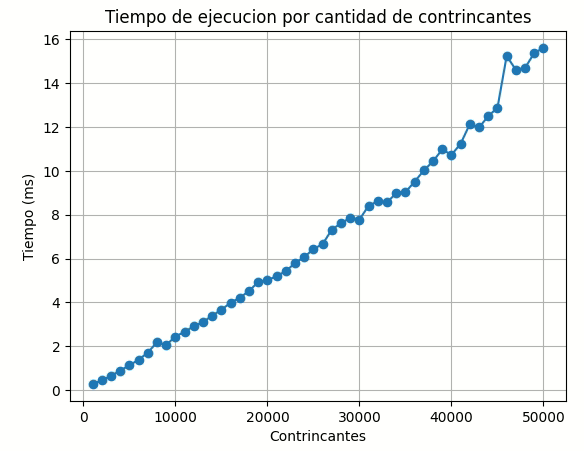
\includegraphics[width=0.65\textwidth]{img/Anomalies.png}
\end{center}
Para esto resolvimos reemplazar esos datos puntuales por un promedio entre el anterior y el siguiente (evitando manualmente situaciones donde más de dos data points seguidos requieren este ajuste):
\begin{lstlisting}[language=Python]
for i in range(1, len(resultado) -1):
    medida_anterior = resultado[i-1][1]
    medida = resultado[i][1]
    medida_siguiente = resultado[i+1][1]

    if medida <= medida_anterior or medida >= medida_siguiente:
        medida_aproximada = (medida_anterior + medida_siguiente)/2
        resultado[i] = (resultado[i][0], round(medida_aproximada, 2))
\end{lstlisting}
Esto nos dejaba con gráficos como el siguiente:
\begin{center}
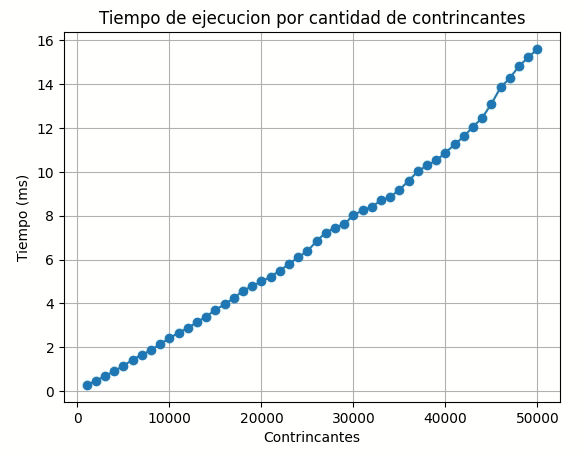
\includegraphics[width=0.65\textwidth]{img/Anomalies2.png}
\end{center}

\subsubsection{Suavizado de la curva}
Como el gráfico post corrección de anomalías seguía siendo un poco irregular, finalmente decidimos aplicar un suavizado a los datos para poder obtener una curva promedio entre los mismos:
\begin{lstlisting}[language=Python]
for i in range(1, len(resultado) -1):
    medida_anterior = resultado[i-1][1]
    medida = resultado[i][1]
    medida_siguiente = resultado[i+1][1]

    medida_aproximada = (medida_anterior + medida_siguiente)/2
    resultado[i] = (resultado[i][0], round(medida_aproximada, 2))
\end{lstlisting}
Esto nos permitió graficar curvas más suaves y fáciles de comparar:
\begin{center}
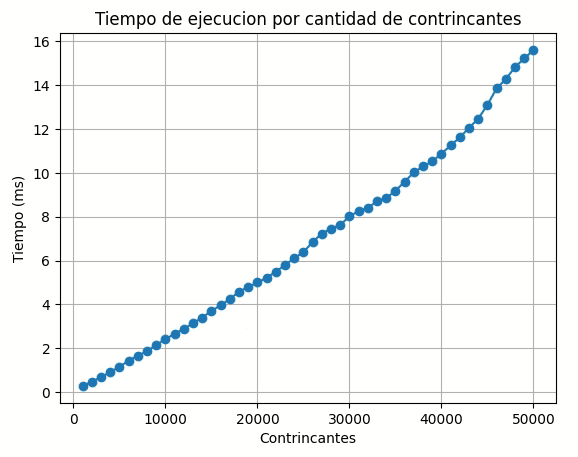
\includegraphics[width=0.7\textwidth]{img/Smoothed.png}
\end{center}

\subsection{Cálculo de curva $k n \log (n)$}

Finalmente, nos quedaba graficar una curva $n \log (n)$ para poder comparar visualmente con la curva de tiempos de ejecución de nuestro algoritmo.

Inicialmente, nos encontramos con la realidad de que la curva $n \log (n)$ se graficaba en varios órdenes de magnitud más altos que nuestra curva de tiempos de ejecución. En parte, esto se debió a una cuestión de unidades ($n \log (n)$ devuelve un número sin unidad que intentamos comparar contra milisegundos) y, en otra parte, porque lo que llamamos $O(1)$ en notación Big O en realidad puede representar una cantidad arbitraria de tiempo.

En base a esto, fue necesario sumar el coeficiente $k$ a la fórmula para llevar la curva a la escala de nuestra curva de resultados y finalmente poder hacer la comparación.

Como resultado, la curva se creó de la siguiente manera:

\begin{lstlisting}[language=Python]
contrincantes = [analisis[0] for analisis in resultado]
tiempos = [analisis[1] for analisis in resultado]

prom_contrincantes = np.mean(contrincantes)
prom_tiempos = np.mean(tiempos)
k = prom_tiempos / (prom_contrincantes * np.log(prom_contrincantes))
print(f"K estimado en {k}")

tiempos_esperados = [k * n * np.log2(n) for n in contrincantes]
\end{lstlisting}

Esto permitió auto ajustar el $k$ de la curva para que siempre sea comparable al resultado de nuestro análisis. En los casos en que se necesitó hacer una comparativa entre distintas corridas, se fijó el valor de $k$ manualmente con el valor resultante de la primera ejecución (para lograr la misma escala en la curva en todos los gráficos a comparar).
\begin{center}
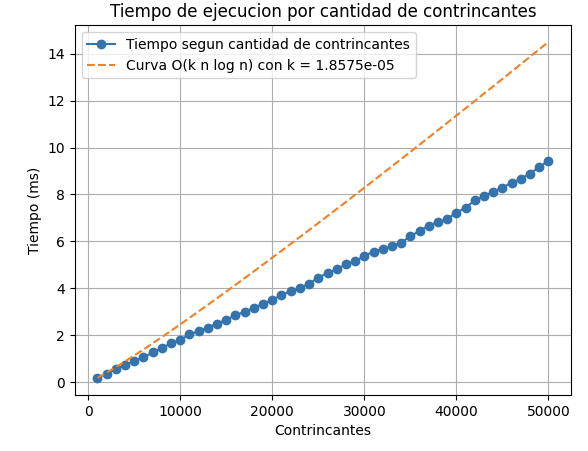
\includegraphics[width=0.7\textwidth]{img/Kcurve.png}
\end{center}
\section{Resultados}

Para corroborar nuestro análisis teórico de la complejidad, generamos varias series de archivos con grandes volúmenes de datos y medimos el tiempo que tarda el algoritmo en procesar cada uno.

Si bien los tiempos de ejecución pueden variar según los recursos de la computadora y pueden verse afectados por motivos externos a la ejecución del algoritmo, verificamos que para distintos $N$, la curva observable se mantuvo comparable a la curva $k n \log (n)$ (ajustando el $k$ para poder compararla cercanamente):
\begin{center}
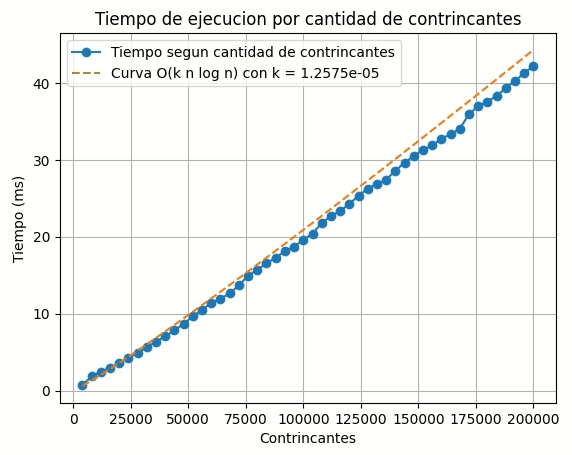
\includegraphics[width=0.7\textwidth]{img/Results.png}
\end{center}
\subsection{Variación de $S_i$ y $A_i$}

Un punto que sí descubrimos mientras realizamos las mediciones es la diferencia que hace el largo de los valores $S_i$ y $A_i$ dentro de los archivos en los tiempos de ejecución.

Por ejemplo, en los siguientes gráficos se puede observar una diferencia mayor al 30% en el tiempo de ejecución entre tener valores que van desde 1 a 1,000,000 a tener valores que van desde 1 a 10:
\begin{center}
\textbf{Con $S_i$ y $A_i$ entre 1 y 1,000,000}

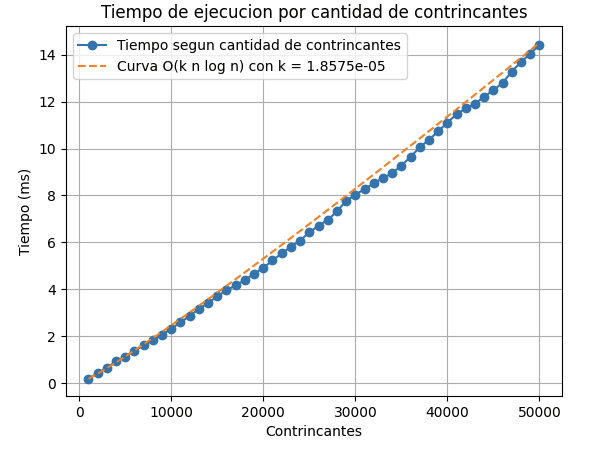
\includegraphics[width=0.8\textwidth]{img/VariationHigh.png}

\textbf{Con $S_i$ y $A_i$ entre 1 y 100}

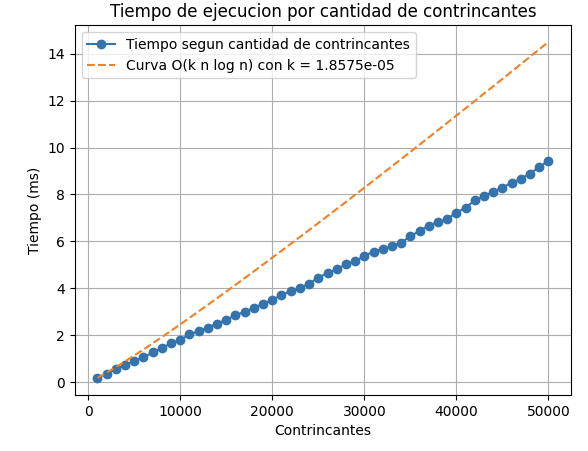
\includegraphics[width=0.8\textwidth]{img/VariationLow.png}
\end{center}
\newpage
\section{Conclusiones}
Primero, podemos concluir que la solución al problema corresponde a un algoritmo Greedy por la aplicación de una regla sencilla que permite encontrar la solución óptima por medio de la búsqueda de óptimos locales. Pudiendo demonstrar que esta solución es optima a traves de la inducción.

Segundo, Francia.
\begin{center}

\includegraphics[width=0.7\textwidth]{img/Campeones.jpeg}
\end{center}

Tercero, por otra parte, y en un tono mas serio, también corroboramos que los tiempos de ejecución se comportaban de la manera esperada según la complejidad que habíamos calculado $O(n \log n)$.

Finalmente, encontramos una diferencia en los tiempos de ejecución del algoritmo en base a los valores de $S_i$ y $A_i$ que llevo a dejar bien en claro lo que cambia entre el teorico $O(n \log n)$ y el $k n \log n$ que se encuentra en la realidad. Resaltando la trampa que puede ser ignorar el factor k (correspondiente a los tiempos "fijos" de ejecucion) a la hora de considerar la complejidad de un algoritmo.

\end{document}

\documentclass{article}
\usepackage{amsmath}
